% 18 variables in here:
% h_1 = 10.0, h_2 = 12.0, h_3 = 7.0, h_4 = 15.0, h_5 = 11.0, h_6 = 9.0, ux_1 = -1.0, ux_2 = 2.0, ux_3 = -3.0, ux_4 = 4.0, ux_5 = -5.0, ux_6 = 6.0, uy_1 = 1.0, uy_2 = -2.0, uy_3 = 3.0, uy_4 = -4.0, uy_5 = 5.0, uy_6 = -6.0
\begin{figure}[h!]
\centering
  \subfloat[] {
    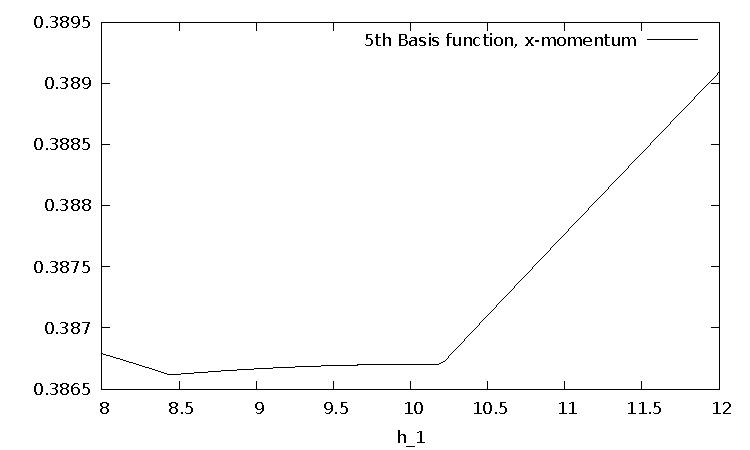
\includegraphics[scale=\zoomfactor]{{{ord2_magnitude_comparison_heights_10_momentums/y_12.0_7.0_15.0_11.0_9.0_-1.0_2.0_-3.0_4.0_-5.0_6.0_1.0_-2.0_3.0_-4.0_5.0_-6.0f08}}}
  }
  \subfloat[] {
    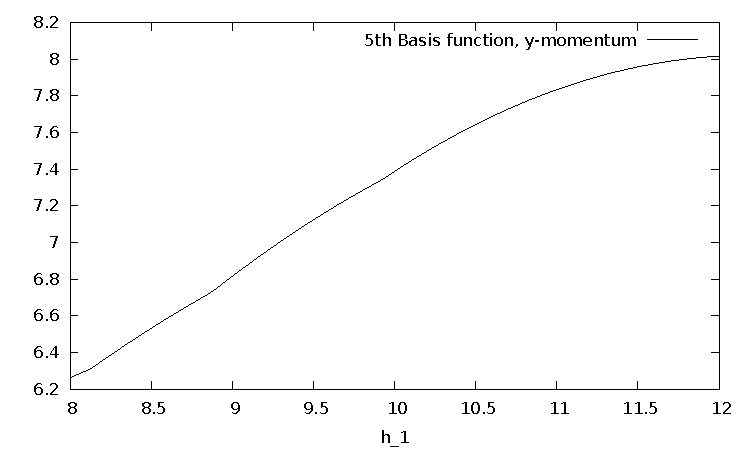
\includegraphics[scale=\zoomfactor]{{{ord2_magnitude_comparison_heights_10_momentums/y_12.0_7.0_15.0_11.0_9.0_-1.0_2.0_-3.0_4.0_-5.0_6.0_1.0_-2.0_3.0_-4.0_5.0_-6.0f09}}}
  }
\caption{}
\label{fig:ord2_magnitude_comparison_heights_10_momentums}
\end{figure}

%%% Local Variables:
%%% TeX-master: "../results.tex"
%%% End:
